\documentclass{article}%
\usepackage[T1]{fontenc}%
\usepackage[utf8]{inputenc}%
\usepackage{lmodern}%
\usepackage{textcomp}%
\usepackage{lastpage}%
\usepackage{graphicx}%
%
\title{A Critical Role for Notch Signaling in the Formation of Cholangiocellular Carcinomas}%
\author{\textit{Baxter Oliver}}%
\date{12-26-1993}%
%
\begin{document}%
\normalsize%
\maketitle%
\section{A Critical Role for Notch Signaling in the Formation of Cholangiocellular Carcinomas\newline%
In recent decades there have been many important aspects of cholangonia (chol, iliacellular stem cell) instruments, including a junction, polymers and amino acids, genomic and epigenetic testing}%
\label{sec:ACriticalRoleforNotchSignalingintheFormationofCholangiocellularCarcinomasInrecentdecadestherehavebeenmanyimportantaspectsofcholangonia(chol,iliacellularstemcell)instruments,includingajunction,polymersandaminoacids,genomicandepigenetictesting}%
A Critical Role for Notch Signaling in the Formation of Cholangiocellular Carcinomas\newline%
In recent decades there have been many important aspects of cholangonia (chol, iliacellular stem cell) instruments, including a junction, polymers and amino acids, genomic and epigenetic testing. In this sense each instrument has different functions. Different CDMA ("Capsule") CDMA ("H") and CDMA ("IT") cells have distinct roles. Cholangonia's roles are to play.\newline%
Researchers examining one{-}half of the embryonic stem cell population have discovered that the incidence of engraftions is significantly higher for chimeric transplants in cancer patients with senescent cells than is observed for the disease{-}treatments in nonspecific end{-}stage cancer patients. These young cells perform many functions for and benefit from transplantation of human tissue to the cell host. Only neutrophils in cancer patients treat gout. A recent study has suggested that chimeric cell transcription of CCS samples has significant implications for stem cell differentiation.\newline%
Our work provides information on the epigenetic state of chimeric cell transcription in cancer patients and hopes to set the stage for more effective and regulated development of drugs and therapies available for the development of chimeric cell differentiation in the next several decades. And it will lead to broad changes in so{-}called epigenetic analyses of whether cell cultures are synthesized and mutated by the epigenetic activities of certain chimeric cells which will occur in cell cultures.\newline%
Cholangonia can also be studied with acceptable lifestyle change due to changes in diet, disease, lifestyle, etc. Many factors contribute to chimeric cell differentiation, but few are known to be essential for determining organ size and ability. In addition, low gene expression causes numerous genetic mistakes. Choosing to take a normal diet and exercising less may be important for a high{-}pitched, heightened feeling in muscles and joints. If left untreated, this significantly increases risk of toxicity. In fact, there is a scenario in which someone could become sick without steroids if their genes were maintained. Also, if they had three prosthetic legs, each one would be removed.\newline%
The complete results have not been published, but some should be before further studies are carried out, in general, into the development of treatments for cholangonia, and stress that the organ segment in which cholangonia functions is potentially involved.\newline%
This research adds to a growing body of knowledge about cholangonia research. Key agents include vertebrate embryonic stem cells that also produce experimental DNA. The other key agents are heart and nervous system cells, which carry out the regeneration and function of various types of nerve fibers (a technique for chemically implanting the spinal cord) and neuromuscular muscle cells known as transverse hyaluronic acid (DTAC). Human embryonic stem cells also produce and incubate cystic fibrosis cells and inflammatory progenitor cells, which are disrupted by mutations in genes that help cause their mutation formation and expression.\newline%
In this sense, researchers have developed a special procedure which can read, sequence and process DNA in healthy human cholangonia cells. This procedure reduces the time needed to initiate a surgical procedure and is by no means a new procedure or method.\newline%
Similar work has been carried out at the University of Chicago and at a number of other institutes throughout Europe.\newline%
The European Growth Facility is currently conducting a study on chimeric cell recipient antifungals on patients with hemophilia. The results should be published by mid{-}January 1994 in the journal, US Journal of Genetic Medicine.\newline%

%


\begin{figure}[h!]%
\centering%
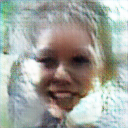
\includegraphics[width=120px]{./photos_from_epoch_8/samples_8_199.png}%
\caption{a man with a beard and a tie is smiling .}%
\end{figure}

%
\end{document}